% !TEX spellcheck = en_US



% ~~~~~~~~~~~~~~~~~~~~~~~~~~~~~~~~~~~~~~~ V
% (NC) 2026 Haluk Bingol
% github.com/halukbingol/LaTeX-Templates
%
% Licensees may copy, distribute, display, and perform the work and make derivative works 
% and remixes based on it only for non-commercial purposes. 
% ~~~~~~~~~~~~~~~~~~~~~~~~~~~~~~~~~~~~~~~ A



% =====================================================================
%  Introduction to Eclipse
%  ---------------------------------------------------------------------
%  Built on hbCisLaTeXTemplate.tex. Every program and its output are read
%  from codeoutput/ (nothing is copied into this .tex):
%     codeoutput/<Name>.java   the program
%     codeoutput/<Name>.in     keyboard input (optional)
%     codeoutput/<Name>.args   program arguments (optional)
%     codeoutput/<Name>.txt    what it printed, made by:  sh run_examples.sh
%  The Eclipse windows are drawn as TikZ schematics, not screenshots.
% =====================================================================

\documentclass[aspectratio=169,10pt,compress]{beamer}

\useoutertheme{split}
\useinnertheme{rounded}
\usecolortheme{whale}
\usecolortheme{orchid}
\setbeamertemplate{blocks}[rounded]
\setbeamertemplate{navigation symbols}{}
% "i / N" on every frame comes from hblibPresentation.sty (\insertshorttitle)

\usepackage[T1]{fontenc}
\usepackage{lmodern}
\usepackage{xcolor}
\usepackage{booktabs}
\usepackage{array}
\usepackage{amssymb}


%\usepackage{hblibCodeoutput}   % lib code + output macros: \lstcode, \lstcodedown, ...
%\usepackage{hblibPresentation}   % lib pesentation libray



% ~~~~~~~~~~~~~~~~~~~~~~~~~~~~~~~~~~~~~~~~~~~~~~~~~~~~~~~~~~~~~~~~~ V hblib
	\usepackage{../../zCisLaTeXTemplate/hblibCodeoutput} % lib code + output macros: \lstcode, \lstcodedown,
	\usepackage{../../zCisLaTeXTemplate/hblibPresentation} % lib pesentation libray (loads algorithm2e)
% ~~~~~~~~~~~~~~~~~~~~~~~~~~~~~~~~~~~~~~~~~~~~~~~~~~~~~~~~~~~~~~~~~ A hblib



\newcolumntype{L}[1]{>{\raggedright\arraybackslash}p{#1}}

\definecolor{gitred}{RGB}{240,80,50}
\newcommand{\cmd}[1]{\texttt{\color{gitred}#1}}

% ---------------------------------------------------------------------
%  Eclipse-specific helpers
% ---------------------------------------------------------------------
\definecolor{eclpane}{RGB}{246,247,250}
\definecolor{eclbar}{RGB}{226,229,236}
\definecolor{ecltab}{RGB}{205,215,235}
\definecolor{eclcur}{RGB}{214,235,200}
\newcommand{\menu}[1]{\textsf{\textbf{#1}}}                      % a menu path
\newcommand{\key}[1]{\tikz[baseline=(k.base)]\node[draw, rounded corners=1.5pt, inner sep=1.5pt,
  fill=gray!8, font=\ttfamily\scriptsize](k){#1};}               % a keyboard key
\newcommand{\kk}[2]{\key{#1}\,{\scriptsize/}\,\key{#2}}           % Windows / macOS keys
\newcommand{\callout}[1]{\tikz[baseline=(c.base)]\node[circle, fill=orange, text=white,
  inner sep=0.8pt, font=\bfseries\tiny](c){#1};}                 % a numbered marker
\newcommand{\tree}{$\triangledown$}                              % open tree node
\newcommand{\treec}{$\triangleright$}                            % closed tree node

\tikzset{
  ewin/.style={draw=gray!70, thick, rounded corners=3pt, fill=white},
  epane/.style={draw=gray!60, fill=eclpane},
  etab/.style={draw=gray!60, fill=ecltab, font=\sffamily\tiny, inner sep=1.5pt, anchor=south west},
  etxt/.style={font=\ttfamily\tiny, anchor=north west, inner sep=0.5pt, align=left},
  ecall/.style={circle, fill=orange, text=white, inner sep=0.8pt, font=\bfseries\scriptsize}
}

% ---------------------------------------------------------------------
\title{Introduction to Eclipse}
\subtitle{Writing, Running and Debugging Java in an IDE}
\author[Bingol]{Haluk O. Bingol}

\institute[FCIS]{
    Faculty of Computer and Information Sciences\\
    Yeditepe University
}
\date{
	{\tiny \hbTimeStamp}
}

\begin{document}




% ~~~~~~~~~~~~~~~~~~~~~~~~~~~~~~~~~~~~~~ V frm
\begin{frame}[t,fragile]
  \titlepage
\end{frame}
% ~~~~~~~~~~~~~~~~~~~~~~~~~~~~~~~~~~~~~~ A frm




% ~~~~~~~~~~~~~~~~~~~~~~~~~~~~~~~~~~~~~~ V frm
\begin{frame}[t,fragile] \frametitle{Outline}
  \begin{columns}[T]
    \begin{column}{0.5\textwidth}
      \tableofcontents[sections={1-4}, hideallsubsections]
    \end{column}
    \begin{column}{0.5\textwidth}
      \tableofcontents[sections={5-8}, hideallsubsections]
    \end{column}
  \end{columns}
\end{frame}
% ~~~~~~~~~~~~~~~~~~~~~~~~~~~~~~~~~~~~~~ A frm

% ~~~~~~~~~~~~~~~~~~~~~~~~~~~~~~~~~~~~~~ V
\hSection[Intro]{What Is Eclipse?}{}{}
% ~~~~~~~~~~~~~~~~~~~~~~~~~~~~~~~~~~~~~~ A

% ~~~~~~~~~~~~~~~~~~~~~~~~~~~~~~~~~~~~~~ V
\subsection[IDE]{Why an IDE?}
% ~~~~~~~~~~~~~~~~~~~~~~~~~~~~~~~~~~~~~~ A




% ~~~~~~~~~~~~~~~~~~~~~~~~~~~~~~~~~~~~~~ V frm
\begin{frame}[t,fragile] \frametitle{Why an IDE?}
  An \textbf{IDE} (Integrated Development Environment) puts everything you need in one window:

  \vspace{0.3em}
  \begin{columns}[T]
    \begin{column}{0.48\textwidth}
      \textbf{Without an IDE}
      \begin{itemize}\small
        \item a text editor for the code
        \item \cmd{javac} and \cmd{java} in a terminal
        \item read error messages, find the line yourself
        \item debug with \texttt{System.out.println}
      \end{itemize}
    \end{column}
    \begin{column}{0.48\textwidth}
      \textbf{With an IDE}
      \begin{itemize}\small
        \item errors are underlined \emph{while you type}
        \item one click (or \kk{Ctrl+F11}{Cmd+Shift+F11}) compiles and runs
        \item code completion, quick fixes, refactoring
        \item a real \textbf{debugger}: pause, step, inspect variables
      \end{itemize}
    \end{column}
  \end{columns}

  \vspace{0.6em}
  \begin{block}{Eclipse}
    \small A free, open-source IDE from the Eclipse Foundation, started at IBM in 2001.
    Written in Java, best known for Java, and extensible with plug-ins
    (\menu{Help $\rightarrow$ Eclipse Marketplace}). Other popular Java IDEs: IntelliJ IDEA, VS Code, NetBeans.
  \end{block}
\end{frame}
% ~~~~~~~~~~~~~~~~~~~~~~~~~~~~~~~~~~~~~~ A frm

% ~~~~~~~~~~~~~~~~~~~~~~~~~~~~~~~~~~~~~~ V
\subsection[Windows]{Installing on Windows}
% ~~~~~~~~~~~~~~~~~~~~~~~~~~~~~~~~~~~~~~ A




% ~~~~~~~~~~~~~~~~~~~~~~~~~~~~~~~~~~~~~~ V frm
\begin{frame}[t,fragile] \frametitle{Installing on Windows}
  \begin{columns}[T]
    \begin{column}{0.48\textwidth}
      \textbf{1. Java (JDK)}
      \begin{enumerate}\small
        \item Go to \texttt{adoptium.net}, choose \textbf{Temurin}, an LTS version (21 or 25), \textbf{Windows x64}, \textbf{.msi}
        \item Run the installer. In \emph{Custom Setup} turn on \textbf{Set JAVA\_HOME variable}
              (and keep \emph{Add to PATH})
        \item Open \textbf{PowerShell} or \textbf{Command Prompt} and check:\\
              \cmd{java -version}
      \end{enumerate}
    \end{column}
    \begin{column}{0.48\textwidth}
      \textbf{2. Eclipse}
      \begin{enumerate}\small
        \item From \texttt{eclipse.org/downloads} download the \textbf{Eclipse Installer} (\texttt{.exe})
        \item Run it and choose \textbf{Eclipse IDE for Java Developers}
        \item Keep the suggested folder, e.g.\\ \texttt{C:\textbackslash Users\textbackslash you\textbackslash eclipse\textbackslash \dots}
        \item Tick \emph{create start menu entry} and \emph{create desktop shortcut}, then \menu{Install} and \menu{Launch}
      \end{enumerate}
      \small If Windows asks for permission or shows a security warning, allow the installer to run.
    \end{column}
  \end{columns}
\end{frame}
% ~~~~~~~~~~~~~~~~~~~~~~~~~~~~~~~~~~~~~~ A frm

% ~~~~~~~~~~~~~~~~~~~~~~~~~~~~~~~~~~~~~~ V
\subsection[macOS]{Installing on macOS}
% ~~~~~~~~~~~~~~~~~~~~~~~~~~~~~~~~~~~~~~ A




% ~~~~~~~~~~~~~~~~~~~~~~~~~~~~~~~~~~~~~~ V frm
\begin{frame}[t,fragile] \frametitle{Installing on macOS}
  \begin{columns}[T]
    \begin{column}{0.48\textwidth}
      \textbf{1. Java (JDK)}
      \begin{enumerate}\small
        \item Which chip? \menu{Apple menu $\rightarrow$ About This Mac}:
              \textbf{Apple M1/M2/\dots} $\Rightarrow$ \textbf{aarch64}; \textbf{Intel} $\Rightarrow$ \textbf{x64}
        \item From \texttt{adoptium.net} download Temurin (21 or 25), \textbf{macOS}, your chip, \textbf{.pkg}, and run it
        \item Or, with Homebrew: \cmd{brew install --cask temurin}
        \item Open \textbf{Terminal} and check: \cmd{java -version}
      \end{enumerate}
    \end{column}
    \begin{column}{0.48\textwidth}
      \textbf{2. Eclipse}
      \begin{enumerate}\small
        \item From \texttt{eclipse.org/downloads} download \textbf{Eclipse IDE for Java Developers}
              as a \texttt{.dmg} for your chip (\textbf{AArch64} or \textbf{x86\_64})
        \item Open the \texttt{.dmg} and drag \textbf{Eclipse} into \textbf{Applications}
        \item Start it from Applications or Launchpad. The first time, macOS asks if you
              want to open an app downloaded from the internet: click \menu{Open}
      \end{enumerate}
      \small JDKs are installed in \texttt{/Library/Java/JavaVirtualMachines/}.
    \end{column}
  \end{columns}
\end{frame}
% ~~~~~~~~~~~~~~~~~~~~~~~~~~~~~~~~~~~~~~ A frm

% ~~~~~~~~~~~~~~~~~~~~~~~~~~~~~~~~~~~~~~ V
\subsection[Start]{First start}
% ~~~~~~~~~~~~~~~~~~~~~~~~~~~~~~~~~~~~~~ A




% ~~~~~~~~~~~~~~~~~~~~~~~~~~~~~~~~~~~~~~ V frm
\begin{frame}[t,fragile] \frametitle{First start (Windows and macOS)}
  \begin{columns}[T]
    \begin{column}{0.52\textwidth}
      \begin{enumerate}\small
        \item Eclipse asks for a \textbf{workspace} folder. The default is
              \begin{itemize}
                \item Windows: \texttt{C:\textbackslash Users\textbackslash you\textbackslash eclipse-workspace}
                \item macOS: \texttt{/Users/you/eclipse-workspace}
              \end{itemize}
        \item Close the \emph{Welcome} tab
        \item Check that Eclipse uses your JDK:
              \begin{itemize}
                \item Windows: \menu{Window $\rightarrow$ Preferences $\rightarrow$ Java $\rightarrow$ Installed JREs}
                \item macOS: \menu{Eclipse $\rightarrow$ Settings\dots{} $\rightarrow$ Java $\rightarrow$ Installed JREs}
                      (\menu{Preferences\dots} in older releases)
              \end{itemize}
      \end{enumerate}
    \end{column}
    \begin{column}{0.44\textwidth}
      \begin{alertblock}{Workspace}
        \small Use one workspace per course. Don't put it in a folder synced by
        \textbf{OneDrive} (Windows) or \textbf{iCloud Desktop \& Documents} (macOS):
        syncing can corrupt Eclipse's files.
      \end{alertblock}
      \begin{block}{Releases}
        \small Eclipse ships four releases a year, named by year and month
        (e.g.\ \texttt{2026-09}). Any recent release works for this course.
      \end{block}
    \end{column}
  \end{columns}
\end{frame}
% ~~~~~~~~~~~~~~~~~~~~~~~~~~~~~~~~~~~~~~ A frm

% ~~~~~~~~~~~~~~~~~~~~~~~~~~~~~~~~~~~~~~ V
\subsection[Conventions]{Windows vs macOS}
% ~~~~~~~~~~~~~~~~~~~~~~~~~~~~~~~~~~~~~~ A




% ~~~~~~~~~~~~~~~~~~~~~~~~~~~~~~~~~~~~~~ V frm
\begin{frame}[t,fragile] \frametitle{Windows vs macOS: what changes}
  \begin{columns}[T]
    \begin{column}{0.56\textwidth}
      \small
      \begin{tabular}{@{}L{0.3\textwidth}L{0.32\textwidth}L{0.32\textwidth}@{}}
        \toprule
        & \textbf{Windows} & \textbf{macOS} \\
        \midrule
        Main modifier   & \key{Ctrl}         & \key{Cmd} \\
        Second modifier & \key{Alt}          & \key{Option} \\
        Enter           & \key{Enter}        & \key{Return} \\
        Right-click     & right mouse button & \key{Ctrl}-click, or two-finger click \\
        Settings        & \menu{Window $\rightarrow$ Preferences} & \menu{Eclipse $\rightarrow$ Settings\dots} \\
        Paths           & \texttt{C:\textbackslash Users\textbackslash you\textbackslash \dots} & \texttt{/Users/you/\dots} \\
        Command line    & PowerShell, Command Prompt & Terminal \\
        \bottomrule
      \end{tabular}
    \end{column}
    \begin{column}{0.4\textwidth}
      \begin{block}{In these slides}
        \small Shortcuts are written as \textbf{Windows / macOS}, e.g.\ \kk{Ctrl+1}{Cmd+1}.
      \end{block}
      \begin{alertblock}{Not just Ctrl $\rightarrow$ Cmd}
        \small
        \begin{itemize}
          \item Run: \kk{Ctrl+F11}{Cmd+Shift+F11}
          \item Debug: \kk{F11}{Cmd+F11}
          \item Content assist is \key{Ctrl+Space} on \emph{both}
          \item On many Mac keyboards, \key{F3}, \key{F5}, \dots{} need \key{fn}
        \end{itemize}
      \end{alertblock}
    \end{column}
  \end{columns}
\end{frame}
% ~~~~~~~~~~~~~~~~~~~~~~~~~~~~~~~~~~~~~~ A frm

% ~~~~~~~~~~~~~~~~~~~~~~~~~~~~~~~~~~~~~~ V
\hSection[Workbench]{The Workbench}{}{}
% ~~~~~~~~~~~~~~~~~~~~~~~~~~~~~~~~~~~~~~ A

% ~~~~~~~~~~~~~~~~~~~~~~~~~~~~~~~~~~~~~~ V
\subsection[Window]{The Eclipse window}
% ~~~~~~~~~~~~~~~~~~~~~~~~~~~~~~~~~~~~~~ A




% ~~~~~~~~~~~~~~~~~~~~~~~~~~~~~~~~~~~~~~ V frm
\begin{frame}[t,fragile] \frametitle{The Eclipse window (Java perspective)}
  \begin{center}
  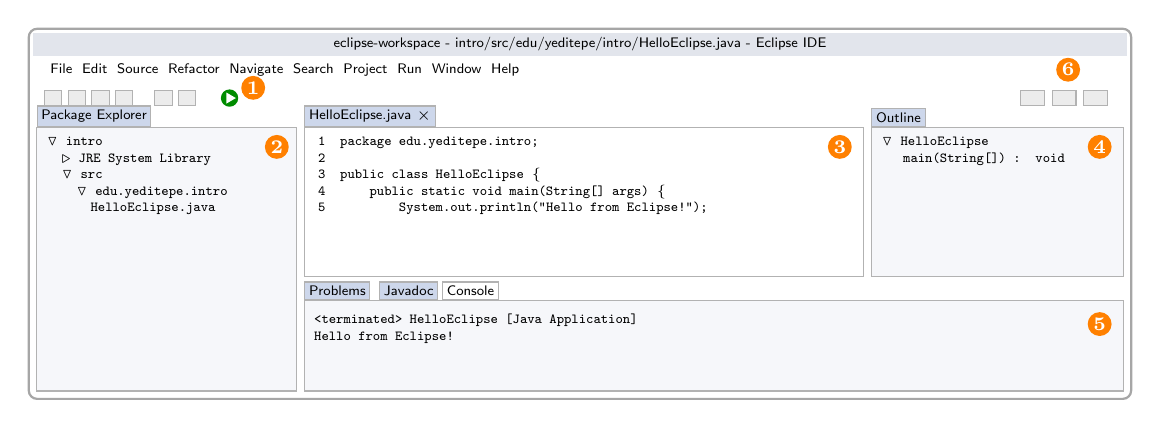
\begin{tikzpicture}[x=1cm, y=1cm]
    % window, title, menu, toolbar
    \draw[ewin] (0,0) rectangle (14,4.7);
    \fill[eclbar] (0.05,4.35) rectangle (13.95,4.65);
    \node[font=\sffamily\tiny] at (7,4.5) {eclipse-workspace - intro/src/edu/yeditepe/intro/HelloEclipse.java - Eclipse IDE};
    \node[font=\sffamily\tiny, anchor=west] at (0.15,4.18) {File\ \ Edit\ \ Source\ \ Refactor\ \ Navigate\ \ Search\ \ Project\ \ Run\ \ Window\ \ Help};
    \foreach \x in {0.2,0.5,0.8,1.1,1.6,1.9} \draw[gray!60, fill=gray!15] (\x,3.72) rectangle ++(0.22,0.2);
    \fill[green!55!black] (2.55,3.82) circle (0.11);
    \fill[white] (2.51,3.75) -- (2.51,3.89) -- (2.63,3.82) -- cycle;
    \draw[gray!60, fill=gray!15] (12.6,3.72) rectangle ++(0.3,0.2) (13.0,3.72) rectangle ++(0.3,0.2) (13.4,3.72) rectangle ++(0.3,0.2);
    % package explorer
    \draw[epane] (0.1,0.1) rectangle (3.4,3.45);
    \node[etab] at (0.1,3.45) {Package Explorer};
    \node[etxt] at (0.2,3.35) {\tree\ intro\\
      \ \ \treec\ JRE System Library\\
      \ \ \tree\ src\\
      \ \ \ \ \tree\ edu.yeditepe.intro\\
      \ \ \ \ \ \ HelloEclipse.java};
    % editor
    \draw[epane, fill=white] (3.5,1.55) rectangle (10.6,3.45);
    \node[etab] at (3.5,3.45) {HelloEclipse.java $\times$};
    \node[etxt] at (3.65,3.35) {1\ \ package edu.yeditepe.intro;\\
      2\\
      3\ \ public class HelloEclipse \{\\
      4\ \ \ \ \ \ public static void main(String[] args) \{\\
      5\ \ \ \ \ \ \ \ \ \ System.out.println("Hello from Eclipse!");};
    % outline
    \draw[epane] (10.7,1.55) rectangle (13.9,3.45);
    \node[etab] at (10.7,3.45) {Outline};
    \node[etxt] at (10.8,3.35) {\tree\ HelloEclipse\\ \ \ \ main(String[]) : void};
    % bottom views
    \draw[epane] (3.5,0.1) rectangle (13.9,1.25);
    \node[etab] at (3.5,1.25) {Problems};
    \node[etab] at (4.45,1.25) {Javadoc};
    \node[etab, fill=white] at (5.25,1.25) {Console};
    \node[etxt] at (3.6,1.1) {<terminated> HelloEclipse [Java Application]\\ Hello from Eclipse!};
    % callouts
    \node[ecall] at (2.85,3.95) {1};
    \node[ecall] at (3.15,3.2) {2};
    \node[ecall] at (10.3,3.2) {3};
    \node[ecall] at (13.6,3.2) {4};
    \node[ecall] at (13.6,0.95) {5};
    \node[ecall] at (13.2,4.18) {6};
  \end{tikzpicture}
  \end{center}
  \vspace{-0.6em}
  \scriptsize
  \begin{tabular}{@{}l@{\ }L{0.4\textwidth}l@{\ }L{0.45\textwidth}@{}}
    \callout{1} & \textbf{Run} button (green): run the program  & \callout{4} & \textbf{Outline}: classes, fields and methods of this file \\
    \callout{2} & \textbf{Package Explorer}: projects, packages, files & \callout{5} & \textbf{Problems} and \textbf{Console}: errors and program output \\
    \callout{3} & \textbf{Editor}: one tab per open file     & \callout{6} & \textbf{Perspective} switcher (Java, Debug, \dots) \\
  \end{tabular}
\end{frame}
% ~~~~~~~~~~~~~~~~~~~~~~~~~~~~~~~~~~~~~~ A frm

% ~~~~~~~~~~~~~~~~~~~~~~~~~~~~~~~~~~~~~~ V
\subsection[Perspectives]{Views and perspectives}
% ~~~~~~~~~~~~~~~~~~~~~~~~~~~~~~~~~~~~~~ A




% ~~~~~~~~~~~~~~~~~~~~~~~~~~~~~~~~~~~~~~ V frm
\begin{frame}[t,fragile] \frametitle{Views and perspectives}
  \begin{columns}[T]
    \begin{column}{0.5\textwidth}
      \textbf{View}: one panel, e.g.\ Package Explorer, Console, Problems, Outline
      \begin{itemize}\small
        \item open one: \menu{Window $\rightarrow$ Show View}
        \item drag a view's tab to move it
        \item double-click a tab to maximize it
      \end{itemize}
      \vspace{0.4em}
      \textbf{Perspective}: a saved arrangement of views for a task
      \begin{itemize}\small
        \item \textbf{Java}: writing code
        \item \textbf{Debug}: stepping through a running program
        \item switch with the buttons at the top right
      \end{itemize}
    \end{column}
    \begin{column}{0.46\textwidth}
      \begin{alertblock}{Lost a view? Messed up the layout?}
        \small \menu{Window $\rightarrow$ Perspective $\rightarrow$ Reset Perspective\dots}
        puts every view back where it started.
      \end{alertblock}
      \begin{block}{Tip}
        \small \kk{Ctrl+Shift+L}{Cmd+Shift+L} shows a list of all keyboard shortcuts.
        Double-click a view's tab to maximize it; double-click again to restore.
      \end{block}
    \end{column}
  \end{columns}
\end{frame}
% ~~~~~~~~~~~~~~~~~~~~~~~~~~~~~~~~~~~~~~ A frm

% ~~~~~~~~~~~~~~~~~~~~~~~~~~~~~~~~~~~~~~ V
\hSection[FirstProject]{Your First Project}{}{}
% ~~~~~~~~~~~~~~~~~~~~~~~~~~~~~~~~~~~~~~ A

% ~~~~~~~~~~~~~~~~~~~~~~~~~~~~~~~~~~~~~~ V
\subsection[Create]{Creating a project and a class}
% ~~~~~~~~~~~~~~~~~~~~~~~~~~~~~~~~~~~~~~ A




% ~~~~~~~~~~~~~~~~~~~~~~~~~~~~~~~~~~~~~~ V frm
\begin{frame}[t,fragile] \frametitle{Creating a project, a package and a class}
  \begin{columns}[T]
    \begin{column}{0.5\textwidth}
      \textbf{1. Project}: \menu{File $\rightarrow$ New $\rightarrow$ Java Project}
      \begin{itemize}\small
        \item Project name: \texttt{intro}
        \item JRE: your JDK
        \item \textbf{uncheck} \emph{Create module-info.java file} (not needed for small programs)
      \end{itemize}
      \textbf{2. Package}: right-click \texttt{src} $\rightarrow$ \menu{New $\rightarrow$ Package}
      \begin{itemize}\small
        \item Name: \texttt{edu.yeditepe.intro}
        \item lower case, reversed domain name; avoid the \emph{default package}
      \end{itemize}
    \end{column}
    \begin{column}{0.46\textwidth}
      \textbf{3. Class}: right-click the package $\rightarrow$ \menu{New $\rightarrow$ Class}
      \begin{itemize}\small
        \item Name: \texttt{HelloEclipse} (starts with a capital letter)
        \item check \texttt{public static void main(String[] args)}
        \item \menu{Finish}: Eclipse writes the skeleton for you
      \end{itemize}
      \textbf{4. Run}: \kk{Ctrl+F11}{Cmd+Shift+F11}, or the green button, or right-click $\rightarrow$
      \menu{Run As $\rightarrow$ Java Application}
    \end{column}
  \end{columns}
\end{frame}
% ~~~~~~~~~~~~~~~~~~~~~~~~~~~~~~~~~~~~~~ A frm

% ~~~~~~~~~~~~~~~~~~~~~~~~~~~~~~~~~~~~~~ V
\subsection[Hello]{Hello, Eclipse}
% ~~~~~~~~~~~~~~~~~~~~~~~~~~~~~~~~~~~~~~ A




% ~~~~~~~~~~~~~~~~~~~~~~~~~~~~~~~~~~~~~~ V frm
\begin{frame}[t,fragile] \frametitle{Hello, Eclipse}
  \lstcoderight[0.7][basicstyle=\ttfamily\scriptsize][basicstyle=\ttfamily\scriptsize]{codeoutput/HelloEclipse.java}{Java}{codeoutput/HelloEclipse.txt}

  \vspace{0.4em}
  \begin{itemize}\small
    \item The output appears in the \textbf{Console} view, under \texttt{<terminated> HelloEclipse [Java Application]}
    \item The first line \texttt{package edu.yeditepe.intro;} matches the folder the file is in
    \item Eclipse compiles automatically every time you save (\kk{Ctrl+S}{Cmd+S}): there is no separate \texttt{javac} step
  \end{itemize}
\end{frame}
% ~~~~~~~~~~~~~~~~~~~~~~~~~~~~~~~~~~~~~~ A frm

% ~~~~~~~~~~~~~~~~~~~~~~~~~~~~~~~~~~~~~~ V
\subsection[Folders]{What is on disk}
% ~~~~~~~~~~~~~~~~~~~~~~~~~~~~~~~~~~~~~~ A




% ~~~~~~~~~~~~~~~~~~~~~~~~~~~~~~~~~~~~~~ V frm
\begin{frame}[t,fragile] \frametitle{What Eclipse puts on disk}
  \begin{columns}[T]
    \begin{column}{0.62\textwidth}


% +++++++++++++++++++++++++++++++++++++++ V lst
%: -Lst.
\begin{lstlisting}[language={}, basicstyle=\ttfamily\scriptsize, frame=single, backgroundcolor=\color{codebg}, rulecolor=\color{gray!40}, numbers=none]
eclipse-workspace/              <- the workspace
|-- .metadata/                  <- Eclipse's own settings
`-- intro/                      <- one Java project
    |-- .project                <- project settings
    |-- .classpath              <- libraries, JDK, folders
    |-- src/                    <- your source code
    |   `-- edu/yeditepe/intro/
    |       `-- HelloEclipse.java
    `-- bin/                    <- compiled .class files
        `-- edu/yeditepe/intro/
            `-- HelloEclipse.class
\end{lstlisting}
% +++++++++++++++++++++++++++++++++++++++ A lst


    \end{column}
    \begin{column}{0.35\textwidth}
      \begin{itemize}\small
        \item Each \textbf{package} is a \textbf{folder}: \texttt{edu.yeditepe.intro} is \texttt{edu/yeditepe/intro/}
        \item \texttt{bin/} is rebuilt by Eclipse; never edit it
        \item To hand in or share code, send the \texttt{src/} files, or export the project
        \item On Windows the same folders use \texttt{\textbackslash}: \texttt{src\textbackslash edu\textbackslash yeditepe\textbackslash intro}
      \end{itemize}
    \end{column}
  \end{columns}
\end{frame}
% ~~~~~~~~~~~~~~~~~~~~~~~~~~~~~~~~~~~~~~ A frm

% ~~~~~~~~~~~~~~~~~~~~~~~~~~~~~~~~~~~~~~ V
\hSection[Editing]{Writing Code Faster}{}{}
% ~~~~~~~~~~~~~~~~~~~~~~~~~~~~~~~~~~~~~~ A

% ~~~~~~~~~~~~~~~~~~~~~~~~~~~~~~~~~~~~~~ V
\subsection[Assist]{Content assist and templates}
% ~~~~~~~~~~~~~~~~~~~~~~~~~~~~~~~~~~~~~~ A




% ~~~~~~~~~~~~~~~~~~~~~~~~~~~~~~~~~~~~~~ V frm
\begin{frame}[t,fragile] \frametitle{Content assist and templates: \texttt{Ctrl+Space}}
  \begin{columns}[T]
    \begin{column}{0.48\textwidth}
      \textbf{Content assist}: type part of a name, press \key{Ctrl+Space}
      \begin{itemize}\small
        \item \texttt{Sys} $\rightarrow$ \texttt{System}
        \item \texttt{names.} $\rightarrow$ list of all methods of \texttt{names}
        \item it also adds the needed \texttt{import} line
      \end{itemize}
      \vspace{0.3em}
      \textbf{Templates}: type a keyword, press \key{Ctrl+Space}
    \end{column}
    \begin{column}{0.48\textwidth}
      \small
      \begin{tabular}{@{}ll@{}}
        \toprule
        \textbf{Type} & \textbf{You get} \\
        \midrule
        \texttt{main}   & \texttt{public static void main(String[] args)} \\
        \texttt{sysout} & \texttt{System.out.println();} \\
        \texttt{syserr} & \texttt{System.err.println();} \\
        \texttt{fori}   & a \texttt{for} loop over an index \\
        \texttt{fore}   & an enhanced \texttt{for} loop \\
        \texttt{if}     & an \texttt{if} block \\
        \bottomrule
      \end{tabular}
    \end{column}
  \end{columns}

  \vspace{0.5em}
  \begin{block}{Tip}
    \small After a template expands, press \key{Tab} to jump between the fields you need to fill in.
    See them all in \menu{Preferences} (macOS: \menu{Settings}) $\rightarrow$ \menu{Java $\rightarrow$ Editor $\rightarrow$ Templates}.
  \end{block}
\end{frame}
% ~~~~~~~~~~~~~~~~~~~~~~~~~~~~~~~~~~~~~~ A frm

% ~~~~~~~~~~~~~~~~~~~~~~~~~~~~~~~~~~~~~~ V
\subsection[QuickFix]{Errors and quick fix}
% ~~~~~~~~~~~~~~~~~~~~~~~~~~~~~~~~~~~~~~ A




% ~~~~~~~~~~~~~~~~~~~~~~~~~~~~~~~~~~~~~~ V frm
\begin{frame}[t,fragile] \frametitle{Errors while you type, and Quick Fix: \texttt{Ctrl+1}}
  \begin{columns}[T]
    \begin{column}{0.55\textwidth}
      \lstcode[basicstyle=\ttfamily\scriptsize]{codeoutput/MissingImport.java}{Java}
      \lstoutput[basicstyle=\ttfamily\scriptsize, firstline=1, lastline=5]{codeoutput/MissingImport.txt}
    \end{column}
    \begin{column}{0.42\textwidth}
      \small
      The terminal compiler (\texttt{javac}) only complains after you compile.
      Eclipse marks the problem \textbf{as you type}:
      \begin{itemize}
        \item a red underline and a red marker in the left margin
        \item the message \emph{ArrayList cannot be resolved to a type}
        \item the same entry in the \textbf{Problems} view
      \end{itemize}
      Put the cursor on the error and press \kk{Ctrl+1}{Cmd+1}. Choose
      \emph{Import 'ArrayList' (java.util)} and the error is gone.
    \end{column}
  \end{columns}
\end{frame}
% ~~~~~~~~~~~~~~~~~~~~~~~~~~~~~~~~~~~~~~ A frm

% ~~~~~~~~~~~~~~~~~~~~~~~~~~~~~~~~~~~~~~ V
\subsection[Source]{Source menu}
% ~~~~~~~~~~~~~~~~~~~~~~~~~~~~~~~~~~~~~~ A




% ~~~~~~~~~~~~~~~~~~~~~~~~~~~~~~~~~~~~~~ V frm
\begin{frame}[t,fragile] \frametitle{Let Eclipse write and tidy code}
  \small
  \begin{tabular}{@{}L{0.2\textwidth}L{0.19\textwidth}L{0.21\textwidth}L{0.34\textwidth}@{}}
    \toprule
    \textbf{Action} & \textbf{Windows} & \textbf{macOS} & \textbf{What it does} \\
    \midrule
    Format & \key{Ctrl+Shift+F} & \key{Cmd+Shift+F} & fixes indentation and spacing \\
    Organize Imports & \key{Ctrl+Shift+O} & \key{Cmd+Shift+O} & adds missing, removes unused imports \\
    Toggle Comment & \key{Ctrl+/} & \key{Cmd+/} & comments out the selected lines \\
    Move line up/down & \key{Alt+$\uparrow\downarrow$} & \key{Option+$\uparrow\downarrow$} & moves the current line \\
    Delete line & \key{Ctrl+D} & \key{Cmd+D} & deletes the current line \\
    Generate code & \key{Alt+Shift+S} & \key{Option+Cmd+S} & getters/setters, constructors, \texttt{toString()} \\
    Open declaration & \key{F3} & \key{F3} & jumps to where a name is defined \\
    Quick outline & \key{Ctrl+O} & \key{Cmd+O} & jump to a method in this file \\
    \bottomrule
  \end{tabular}

  \vspace{0.6em}
  \normalsize
  \begin{block}{Habit}
    \small Press \kk{Ctrl+Shift+F}{Cmd+Shift+F} before you hand in code: consistent formatting makes it easier to read and grade.
  \end{block}
\end{frame}
% ~~~~~~~~~~~~~~~~~~~~~~~~~~~~~~~~~~~~~~ A frm

% ~~~~~~~~~~~~~~~~~~~~~~~~~~~~~~~~~~~~~~ V
\subsection[Refactor]{Refactoring}
% ~~~~~~~~~~~~~~~~~~~~~~~~~~~~~~~~~~~~~~ A




% ~~~~~~~~~~~~~~~~~~~~~~~~~~~~~~~~~~~~~~ V frm
\begin{frame}[t,fragile] \frametitle{Refactoring: before}
  \lstcodedown[basicstyle=\ttfamily\scriptsize, firstline=3][basicstyle=\ttfamily\scriptsize]{codeoutput/RefactorBefore.java}{Java}{codeoutput/RefactorBefore.txt}

  \small The same summing loop is written twice, and \texttt{fin} is not a clear name.
\end{frame}
% ~~~~~~~~~~~~~~~~~~~~~~~~~~~~~~~~~~~~~~ A frm




% ~~~~~~~~~~~~~~~~~~~~~~~~~~~~~~~~~~~~~~ V frm
\begin{frame}[t,fragile] \frametitle{Refactoring: after (same output)}
  \lstcodedownstep[basicstyle=\ttfamily\scriptsize, firstline=3][basicstyle=\ttfamily\scriptsize]{codeoutput/RefactorAfter.java}{Java}{codeoutput/RefactorAfter.txt}

  \small Refactoring changes the \emph{structure} of the code, never its \emph{behavior}: the output is identical.
\end{frame}
% ~~~~~~~~~~~~~~~~~~~~~~~~~~~~~~~~~~~~~~ A frm




% ~~~~~~~~~~~~~~~~~~~~~~~~~~~~~~~~~~~~~~ V frm
\begin{frame}[t,fragile] \frametitle{How to do it in Eclipse}
  \begin{enumerate}
    \item \textbf{Extract Method} \kk{Alt+Shift+M}{Option+Cmd+M}: select the summing loop, choose a name
          (\texttt{average}). Eclipse creates the method and passes the array as a parameter.
          Adjust it to return the average, then call it for both arrays.
    \item \textbf{Rename} \kk{Alt+Shift+R}{Option+Cmd+R}: put the cursor on \texttt{fin}, type \texttt{finalExam},
          press \kk{Enter}{Return}. Every use is renamed, and nothing else.
    \item Run again: the output must be \textbf{exactly the same}.
  \end{enumerate}

  \vspace{0.6em}
  \begin{columns}[T]
    \begin{column}{0.48\textwidth}
      \begin{block}{Why not search and replace?}
        \small Refactoring understands Java: renaming \texttt{fin} does not touch \texttt{final}
        or a \texttt{fin} in another method.
      \end{block}
    \end{column}
    \begin{column}{0.48\textwidth}
      \begin{alertblock}{Undo}
        \small \kk{Ctrl+Z}{Cmd+Z} undoes a whole refactoring in one step.
      \end{alertblock}
    \end{column}
  \end{columns}
\end{frame}
% ~~~~~~~~~~~~~~~~~~~~~~~~~~~~~~~~~~~~~~ A frm

% ~~~~~~~~~~~~~~~~~~~~~~~~~~~~~~~~~~~~~~ V
\hSection[Running]{Running Programs}{}{}
% ~~~~~~~~~~~~~~~~~~~~~~~~~~~~~~~~~~~~~~ A

% ~~~~~~~~~~~~~~~~~~~~~~~~~~~~~~~~~~~~~~ V
\subsection[Arguments]{Program arguments}
% ~~~~~~~~~~~~~~~~~~~~~~~~~~~~~~~~~~~~~~ A




% ~~~~~~~~~~~~~~~~~~~~~~~~~~~~~~~~~~~~~~ V frm
\begin{frame}[t,fragile] \frametitle{Program arguments: \texttt{String[] args}}
  \lstcoderight[0.7][basicstyle=\ttfamily\scriptsize][basicstyle=\ttfamily\scriptsize]{codeoutput/Args.java}{Java}{codeoutput/Args.txt}

  \small In PowerShell or Terminal you would type \cmd{java edu.yeditepe.intro.Args Ada 3}. In Eclipse:
  \menu{Run $\rightarrow$ Run Configurations\dots} $\rightarrow$ select \texttt{Args} $\rightarrow$
  \menu{Arguments} tab $\rightarrow$ \emph{Program arguments}: \texttt{Ada 3} $\rightarrow$ \menu{Run}.
  Without arguments, \texttt{args[0]} throws an \texttt{ArrayIndexOutOfBoundsException}.
\end{frame}
% ~~~~~~~~~~~~~~~~~~~~~~~~~~~~~~~~~~~~~~ A frm

% ~~~~~~~~~~~~~~~~~~~~~~~~~~~~~~~~~~~~~~ V
\subsection[Input]{Keyboard input}
% ~~~~~~~~~~~~~~~~~~~~~~~~~~~~~~~~~~~~~~ A




% ~~~~~~~~~~~~~~~~~~~~~~~~~~~~~~~~~~~~~~ V frm
\begin{frame}[t,fragile] \frametitle{Keyboard input in the Console}
  \begin{columns}[T]
    \begin{column}{0.6\textwidth}
      \lstcode[basicstyle=\ttfamily\scriptsize]{codeoutput/ConsoleInput.java}{Java}
    \end{column}
    \begin{column}{0.38\textwidth}
      \lstcode[basicstyle=\ttfamily\scriptsize, numbers=none]{codeoutput/ConsoleInput.in}{}
      \lstoutput[basicstyle=\ttfamily\scriptsize]{codeoutput/ConsoleInput.txt}
      \small Type the input in the \textbf{Console} view and press \kk{Enter}{Return}.
      Eclipse shows what you type in green.
      Here the input came from a file, so it is not echoed.
    \end{column}
  \end{columns}
\end{frame}
% ~~~~~~~~~~~~~~~~~~~~~~~~~~~~~~~~~~~~~~ A frm

% ~~~~~~~~~~~~~~~~~~~~~~~~~~~~~~~~~~~~~~ V
\hSection[Debugging]{Debugging}{}{}
% ~~~~~~~~~~~~~~~~~~~~~~~~~~~~~~~~~~~~~~ A

% ~~~~~~~~~~~~~~~~~~~~~~~~~~~~~~~~~~~~~~ V
\subsection[Bug]{A program with a bug}
% ~~~~~~~~~~~~~~~~~~~~~~~~~~~~~~~~~~~~~~ A




% ~~~~~~~~~~~~~~~~~~~~~~~~~~~~~~~~~~~~~~ V frm
\begin{frame}[t,fragile] \frametitle{A program with a bug}
  \lstcodeoverlaystep[basicstyle=\ttfamily\scriptsize][basicstyle=\ttfamily\scriptsize][0.3\textwidth]{10.6cm,2.2cm}%
    {codeoutput/BuggyAverage.java}{Java}{codeoutput/BuggyAverage.txt}

  \small \only<1>{The average of 85, 90 and 72 should be 82.33. What does this program print?}%
  \only<2>{It prints 54.0. Instead of adding more \texttt{println} lines, let's use the debugger.}
\end{frame}
% ~~~~~~~~~~~~~~~~~~~~~~~~~~~~~~~~~~~~~~ A frm

% ~~~~~~~~~~~~~~~~~~~~~~~~~~~~~~~~~~~~~~ V
\subsection[Breakpoints]{Breakpoints and stepping}
% ~~~~~~~~~~~~~~~~~~~~~~~~~~~~~~~~~~~~~~ A




% ~~~~~~~~~~~~~~~~~~~~~~~~~~~~~~~~~~~~~~ V frm
\begin{frame}[t,fragile] \frametitle{Breakpoints and stepping}
  \begin{columns}[T]
    \begin{column}{0.52\textwidth}
      \begin{enumerate}\small
        \item \textbf{Set a breakpoint}: double-click the left margin of line 7
              (or \kk{Ctrl+Shift+B}{Cmd+Shift+B}). A blue dot appears
        \item \textbf{Start debugging}: \kk{F11}{Cmd+F11}, or right-click $\rightarrow$
              \menu{Debug As $\rightarrow$ Java Application}
        \item Eclipse offers to switch to the \textbf{Debug perspective}: say yes
        \item The program \textbf{pauses} before running line 7
        \item Look at the \textbf{Variables} view, then step
      \end{enumerate}
    \end{column}
    \begin{column}{0.44\textwidth}
      \small
      \begin{tabular}{@{}lL{0.6\textwidth}@{}}
        \toprule
        \textbf{Key} & \textbf{Action} \\
        \midrule
        \key{F6} & \textbf{Step Over}: run this line \\
        \key{F5} & \textbf{Step Into}: go into the method called here \\
        \key{F7} & \textbf{Step Return}: finish this method \\
        \key{F8} & \textbf{Resume}: run to the next breakpoint \\
        \kk{Ctrl+R}{Cmd+R} & run to the line with the cursor \\
        \kk{Ctrl+F2}{Cmd+F2} & \textbf{Terminate} the program \\
        \bottomrule
      \end{tabular}
    \end{column}
  \end{columns}
\end{frame}
% ~~~~~~~~~~~~~~~~~~~~~~~~~~~~~~~~~~~~~~ A frm

% ~~~~~~~~~~~~~~~~~~~~~~~~~~~~~~~~~~~~~~ V
\subsection[Perspective]{The Debug perspective}
% ~~~~~~~~~~~~~~~~~~~~~~~~~~~~~~~~~~~~~~ A




% ~~~~~~~~~~~~~~~~~~~~~~~~~~~~~~~~~~~~~~ V frm
\begin{frame}[t,fragile] \frametitle{The Debug perspective, paused on line 7}
  \begin{center}
  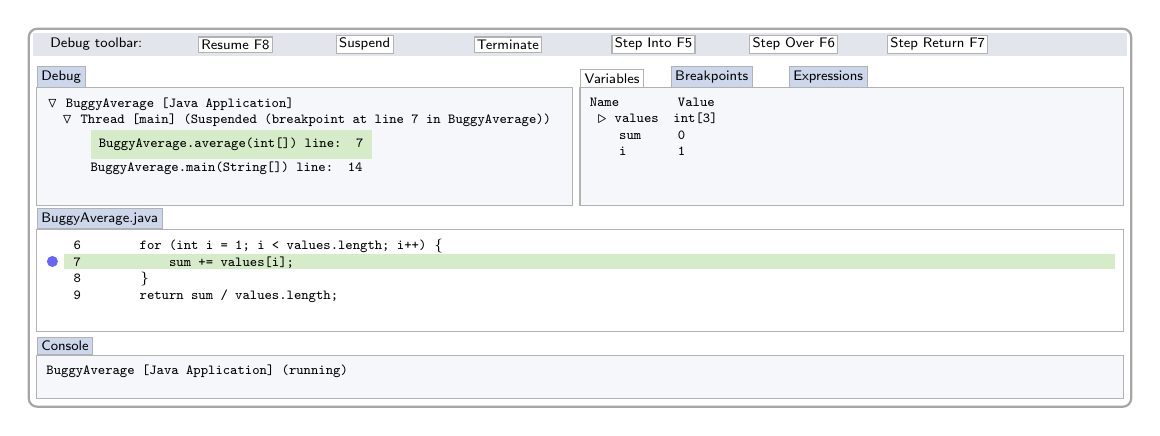
\begin{tikzpicture}[x=1cm, y=1cm]
    \draw[ewin] (0,0) rectangle (14,4.8);
    \fill[eclbar] (0.05,4.45) rectangle (13.95,4.75);
    % debug toolbar
    \node[font=\sffamily\tiny, anchor=west] at (0.15,4.6) {Debug toolbar:};
    \foreach \lbl [count=\i] in {Resume F8, Suspend, Terminate, Step Into F5, Step Over F6, Step Return F7}
      \node[draw=gray!60, fill=white, font=\sffamily\tiny, inner sep=1pt, anchor=west] at (0.4+\i*1.75,4.6) {\lbl};
    % debug view
    \draw[epane] (0.1,2.55) rectangle (6.9,4.05);
    \node[etab] at (0.1,4.05) {Debug};
    \node[etxt] at (0.2,3.95) {\tree\ BuggyAverage [Java Application]\\
      \ \ \tree\ Thread [main] (Suspended (breakpoint at line 7 in BuggyAverage))\\
      \ \ \ \ \ \ \colorbox{eclcur}{BuggyAverage.average(int[]) line: 7}\\
      \ \ \ \ \ \ BuggyAverage.main(String[]) line: 14};
    % variables view
    \draw[epane] (7.0,2.55) rectangle (13.9,4.05);
    \node[etab, fill=white] at (7.0,4.05) {Variables};
    \node[etab] at (8.15,4.05) {Breakpoints};
    \node[etab] at (9.65,4.05) {Expressions};
    \node[etxt] at (7.1,3.95) {Name\ \ \ \ \ \ \ \ Value\\
      \ \treec\ values\ \ int[3]\\
      \ \ \ \ sum\ \ \ \ \ 0\\
      \ \ \ \ i\ \ \ \ \ \ \ 1};
    % editor
    \draw[epane, fill=white] (0.1,0.95) rectangle (13.9,2.25);
    \node[etab] at (0.1,2.25) {BuggyAverage.java};
    \fill[eclcur] (0.45,1.745) rectangle (13.8,1.945);
    \fill[blue!60] (0.3,1.845) circle (0.07);
    \node[etxt] at (0.45,2.15) {\ 6\ \ \ \ \ \ \ \ for (int i = 1; i < values.length; i++) \{\\
      \ 7\ \ \ \ \ \ \ \ \ \ \ \ sum += values[i];\\
      \ 8\ \ \ \ \ \ \ \ \}\\
      \ 9\ \ \ \ \ \ \ \ return sum / values.length;};
    % console
    \draw[epane] (0.1,0.1) rectangle (13.9,0.65);
    \node[etab] at (0.1,0.65) {Console};
    \node[etxt] at (0.2,0.55) {BuggyAverage [Java Application] (running)};
  \end{tikzpicture}
  \end{center}
  \vspace{-0.5em}
  \small The highlighted line is the \textbf{next} line to run. The blue dot is the breakpoint.
  \texttt{i} is already \texttt{1}: the first grade (\texttt{values[0] = 85}) will never be added.
\end{frame}
% ~~~~~~~~~~~~~~~~~~~~~~~~~~~~~~~~~~~~~~ A frm

% ~~~~~~~~~~~~~~~~~~~~~~~~~~~~~~~~~~~~~~ V
\subsection[Trace]{Finding the bug}
% ~~~~~~~~~~~~~~~~~~~~~~~~~~~~~~~~~~~~~~ A




% ~~~~~~~~~~~~~~~~~~~~~~~~~~~~~~~~~~~~~~ V frm
\begin{frame}[t,fragile] \frametitle{Watching the variables}
  \begin{columns}[T]
    \begin{column}{0.5\textwidth}
      Pressing \key{F6} repeatedly, the Variables view shows:

      \vspace{0.4em}
      \small
      \begin{tabular}{@{}lccl@{}}
        \toprule
        \textbf{Paused at} & \texttt{i} & \texttt{sum} & \textbf{Note} \\
        \midrule
        line 7, 1st time & 1 & 0   & \hRemark{\texttt{i} starts at 1} \\
        line 7, 2nd time & 2 & 90  & \\
        line 9           & -- & 162 & $162 = 90 + 72$ \\
        \bottomrule
      \end{tabular}

      \vspace{0.6em}
      \normalsize
      Two bugs:
      \begin{enumerate}\small
        \item the loop skips \texttt{values[0]}
        \item \texttt{162 / 3} is \textbf{integer} division: \texttt{54}, not 54.0 (the conversion
              to \texttt{double} happens too late)
      \end{enumerate}
    \end{column}
    \begin{column}{0.48\textwidth}
      \only<2->{\lstcodedown[basicstyle=\ttfamily\tiny, firstline=4, lastline=10, firstnumber=4][basicstyle=\ttfamily\scriptsize]%
        {codeoutput/FixedAverage.java}{Java}{codeoutput/FixedAverage.txt}}
    \end{column}
  \end{columns}
\end{frame}
% ~~~~~~~~~~~~~~~~~~~~~~~~~~~~~~~~~~~~~~ A frm

% ~~~~~~~~~~~~~~~~~~~~~~~~~~~~~~~~~~~~~~ V
\hSection[More]{More Tools}{}{}
% ~~~~~~~~~~~~~~~~~~~~~~~~~~~~~~~~~~~~~~ A

% ~~~~~~~~~~~~~~~~~~~~~~~~~~~~~~~~~~~~~~ V
\subsection[JUnit]{Unit tests with JUnit}
% ~~~~~~~~~~~~~~~~~~~~~~~~~~~~~~~~~~~~~~ A




% ~~~~~~~~~~~~~~~~~~~~~~~~~~~~~~~~~~~~~~ V frm
\begin{frame}[t,fragile] \frametitle{Unit tests with JUnit}
  \begin{columns}[T]
    \begin{column}{0.56\textwidth}
      \lstcode[basicstyle=\ttfamily\tiny]{codeoutput/test/AverageTest.java}{Java}
    \end{column}
    \begin{column}{0.42\textwidth}
      \begin{enumerate}\small
        \item Right-click the class to test $\rightarrow$ \menu{New $\rightarrow$ JUnit Test Case}
        \item Choose \textbf{JUnit Jupiter} (JUnit 5); accept adding the library to the build path
        \item Write test methods marked \texttt{@Test}
        \item Right-click $\rightarrow$ \menu{Run As $\rightarrow$ JUnit Test}
      \end{enumerate}
      \small The \textbf{JUnit} view shows a \textcolor{green!50!black}{\textbf{green bar}} when every test passes,
      and a \textcolor{red}{\textbf{red bar}} with the failing test and the expected vs.\ actual values otherwise.
      Run it against \texttt{BuggyAverage} and it turns red.
    \end{column}
  \end{columns}
\end{frame}
% ~~~~~~~~~~~~~~~~~~~~~~~~~~~~~~~~~~~~~~ A frm

% ~~~~~~~~~~~~~~~~~~~~~~~~~~~~~~~~~~~~~~ V
\subsection[Git]{Git, import and export}
% ~~~~~~~~~~~~~~~~~~~~~~~~~~~~~~~~~~~~~~ A




% ~~~~~~~~~~~~~~~~~~~~~~~~~~~~~~~~~~~~~~ V frm
\begin{frame}[t,fragile] \frametitle{Git, import and export}
  \begin{columns}[T]
    \begin{column}{0.5\textwidth}
      \textbf{Git} is built in (the EGit plug-in)
      \begin{itemize}\small
        \item clone: \menu{File $\rightarrow$ Import $\rightarrow$ Git $\rightarrow$ Projects from Git}
        \item put a project under Git: right-click $\rightarrow$ \menu{Team $\rightarrow$ Share Project}
        \item stage and commit in the \textbf{Git Staging} view
        \item pull and push from the \menu{Team} menu
      \end{itemize}
      \small The commands are the same ideas as in the Git lectures, just with buttons.
    \end{column}
    \begin{column}{0.46\textwidth}
      \textbf{Sharing projects}
      \begin{itemize}\small
        \item open a project someone gave you:\\
              \menu{File $\rightarrow$ Import $\rightarrow$ General $\rightarrow$ Existing Projects into Workspace}
        \item make a program others can run:\\
              \menu{File $\rightarrow$ Export $\rightarrow$ Java $\rightarrow$ Runnable JAR file},\\
              then in PowerShell / Terminal:\\ \cmd{java -jar intro.jar}
        \item files changed outside Eclipse? select the project and press \key{F5} (Refresh)
      \end{itemize}
    \end{column}
  \end{columns}
\end{frame}
% ~~~~~~~~~~~~~~~~~~~~~~~~~~~~~~~~~~~~~~ A frm

% ~~~~~~~~~~~~~~~~~~~~~~~~~~~~~~~~~~~~~~ V
\hSection[Summary]{Summary}{}{}
% ~~~~~~~~~~~~~~~~~~~~~~~~~~~~~~~~~~~~~~ A

% ~~~~~~~~~~~~~~~~~~~~~~~~~~~~~~~~~~~~~~ V
\subsection[Trouble]{Troubleshooting}
% ~~~~~~~~~~~~~~~~~~~~~~~~~~~~~~~~~~~~~~ A




% ~~~~~~~~~~~~~~~~~~~~~~~~~~~~~~~~~~~~~~ V frm
\begin{frame}[t,fragile] \frametitle{Troubleshooting}
  \small
  \begin{tabular}{@{}L{0.4\textwidth}L{0.54\textwidth}@{}}
    \toprule
    \textbf{Symptom} & \textbf{Try this} \\
    \midrule
    \emph{Selection does not contain a main type} & the class has no \texttt{main} method, or you right-clicked another file \\
    macOS: \key{F5}, \key{F6}, \dots{} do nothing & press \key{fn} too, or turn on \emph{Use F1, F2, etc.\ keys as standard function keys} in System Settings $\rightarrow$ Keyboard \\
    macOS: \key{Ctrl+Space} changes the keyboard language & System Settings $\rightarrow$ Keyboard $\rightarrow$ Keyboard Shortcuts $\rightarrow$ Input Sources: turn off or change that shortcut \\
    A view disappeared & \menu{Window $\rightarrow$ Perspective $\rightarrow$ Reset Perspective} \\
    \emph{Errors exist in required project(s)\dots{} Proceed with launch?} & open the \textbf{Problems} view and fix the red errors first \\
    Red errors everywhere, \texttt{String} not found & \menu{Project $\rightarrow$ Properties $\rightarrow$ Java Build Path $\rightarrow$ Libraries}: add your JDK \\
    Changed files outside Eclipse & select the project, press \key{F5} (Refresh) \\
    Strange errors after an update & \menu{Project $\rightarrow$ Clean\dots} rebuilds everything \\
    Program still running & red square in the Console, or \kk{Ctrl+F2}{Cmd+F2} \\
    \bottomrule
  \end{tabular}
\end{frame}
% ~~~~~~~~~~~~~~~~~~~~~~~~~~~~~~~~~~~~~~ A frm

% ~~~~~~~~~~~~~~~~~~~~~~~~~~~~~~~~~~~~~~ V
\subsection[Shortcuts]{Shortcut cheat sheet}
% ~~~~~~~~~~~~~~~~~~~~~~~~~~~~~~~~~~~~~~ A




% ~~~~~~~~~~~~~~~~~~~~~~~~~~~~~~~~~~~~~~ V frm
\begin{frame}[t,fragile] \frametitle{Shortcut cheat sheet: writing code}
  \small
  \begin{center}
      \begin{tabular}{@{}L{0.36\textwidth}L{0.24\textwidth}L{0.26\textwidth}@{}}
        \toprule
        \textbf{Action} & \textbf{Windows} & \textbf{macOS} \\
        \midrule
        Content assist, templates & \key{Ctrl+Space} & \key{Ctrl+Space} \\
        Quick fix & \key{Ctrl+1} & \key{Cmd+1} \\
        Format & \key{Ctrl+Shift+F} & \key{Cmd+Shift+F} \\
        Organize imports & \key{Ctrl+Shift+O} & \key{Cmd+Shift+O} \\
        Toggle comment & \key{Ctrl+/} & \key{Cmd+/} \\
        Delete line & \key{Ctrl+D} & \key{Cmd+D} \\
        Rename & \key{Alt+Shift+R} & \key{Option+Cmd+R} \\
        Extract method & \key{Alt+Shift+M} & \key{Option+Cmd+M} \\
        Source menu (generate code) & \key{Alt+Shift+S} & \key{Option+Cmd+S} \\
        Save (and compile) & \key{Ctrl+S} & \key{Cmd+S} \\
        Undo & \key{Ctrl+Z} & \key{Cmd+Z} \\
        \bottomrule
      \end{tabular}
  \end{center}
\end{frame}
% ~~~~~~~~~~~~~~~~~~~~~~~~~~~~~~~~~~~~~~ A frm




% ~~~~~~~~~~~~~~~~~~~~~~~~~~~~~~~~~~~~~~ V frm
\begin{frame}[t,fragile] \frametitle{Shortcut cheat sheet: running, debugging, finding}
  \small
  \begin{center}
      \begin{tabular}{@{}L{0.36\textwidth}L{0.24\textwidth}L{0.26\textwidth}@{}}
        \toprule
        \textbf{Action} & \textbf{Windows} & \textbf{macOS} \\
        \midrule
        Run & \key{Ctrl+F11} & \key{Cmd+Shift+F11} \\
        Debug & \key{F11} & \key{Cmd+F11} \\
        Toggle breakpoint & \key{Ctrl+Shift+B} & \key{Cmd+Shift+B} \\
        Step into / over / return & \key{F5 / F6 / F7} & \key{F5 / F6 / F7} \\
        Resume & \key{F8} & \key{F8} \\
        Run to line & \key{Ctrl+R} & \key{Cmd+R} \\
        Terminate & \key{Ctrl+F2} & \key{Cmd+F2} \\
        Open declaration & \key{F3} & \key{F3} \\
        Quick outline & \key{Ctrl+O} & \key{Cmd+O} \\
        Open a class by name & \key{Ctrl+Shift+T} & \key{Cmd+Shift+T} \\
        List all shortcuts & \key{Ctrl+Shift+L} & \key{Cmd+Shift+L} \\
        \bottomrule
      \end{tabular}
  \end{center}

  \vspace{0.2em}
  \small On many Mac keyboards the \key{F} keys need \key{fn} as well.
\end{frame}
% ~~~~~~~~~~~~~~~~~~~~~~~~~~~~~~~~~~~~~~ A frm

% ~~~~~~~~~~~~~~~~~~~~~~~~~~~~~~~~~~~~~~ V
\subsection[Exercises]{Exercises}
% ~~~~~~~~~~~~~~~~~~~~~~~~~~~~~~~~~~~~~~ A




% ~~~~~~~~~~~~~~~~~~~~~~~~~~~~~~~~~~~~~~ V frm
\begin{frame}[t,fragile] \frametitle{Exercises}
  \begin{enumerate}\small
    \item Install Eclipse, create the workspace and the project \texttt{intro}, and run \texttt{HelloEclipse}.
    \item Create a new class using only templates: type \texttt{main} and \texttt{sysout} with \key{Ctrl+Space}.
    \item Delete an \texttt{import} line on purpose, then fix it with \kk{Ctrl+1}{Cmd+1}, and again with \kk{Ctrl+Shift+O}{Cmd+Shift+O}.
    \item Run \texttt{Args} with and without program arguments. Read the exception in the Console and click the
          link in the stack trace to jump to the line.
    \item Debug \texttt{BuggyAverage}: set a breakpoint, step with \key{F6}, and write down \texttt{i} and \texttt{sum}
          after each step. Fix both bugs.
    \item Apply \emph{Extract Method} and \emph{Rename} to one of your own programs; check that the output did not change.
    \item Write a JUnit test for \texttt{average} that fails for \texttt{BuggyAverage} and passes for \texttt{FixedAverage}.
  \end{enumerate}

  \vspace{0.3em}
  \begin{center}
    {\Large \textbf{Questions?}}
  \end{center}
\end{frame}
% ~~~~~~~~~~~~~~~~~~~~~~~~~~~~~~~~~~~~~~ A frm

\end{document}
